\documentclass[conference]{IEEEtran}
\usepackage{graphicx}

% path gambar
\graphicspath{{./picture/}}

% JUDUL %%%%%%%%%%%%%%%%%%%%%%%%%%%%%%%%%%%%%%%%%%%%%%%%%%%%%
\title{Analisis Kekuatan Sinyal Menggunakan InSSIDer}

% PENULIS %%%%%%%%%%%%%%%%%%%%%%%%%%%%%%%%%%%%%%%%%%%%%%%%%%%
\author{Andrian Syah\IEEEauthorrefmark{1}, Hani Khairiyah\IEEEauthorrefmark{2}\\
\textit{Fakultas Teknologi Informasi}\\
\textit{Teknik Komputer}\\
\textit{Institut Teknologi Batam}\\
Batam, Indonesia\\
Email: \{\IEEEauthorrefmark{1}1922009, \IEEEauthorrefmark{2}1922001\}@student.iteba.ac.id}

\begin{document}

% untuk mengeluarkan judul dan author
\maketitle

% ABSTRAK %%%%%%%%%%%%%%%%%%%%%%%%%%%%%%%%%%%%%%%%%%%%%%%%%%
\begin{abstract}
    Analisa Wireless atau jaringan nirkabel menggunakan aplikasi InSSIDer ,
    Mengumpulkan Informasi yang ada pada jaringan Wireless sekitar dan mengambil data 
    untuk dianalisa .
\end{abstract}

% kata kunci %%%%%%%%%%%%%%%%%%%%%%%%%%%%%%%%%%%%%%%%%%%%%%%%
\begin{IEEEkeywords}
    IEEE 802.11,InSSIDer,Wireless
\end{IEEEkeywords}

% pendahuluan %%%%%%%%%%%%%%%%%%%%%%%%%%%%%%%%%%%%%%%%%%%%%%
\section{Pendahuluan}
Seiring berkembang nya zaman Teknologi semakin tidak bisa dihindarkan, 
kita sebagai manusia tidak dapat menghindar dari adanya teknologi tersebut,
banyak nya teknologi membuat banyak hal berubah sehingga menjadikan teknologi tersebut 
adalah bagian dari hidup. salah satu dari teknologi tersebut adalah teknologi jaringan nirkabel
atau bisa disebut teknologi jaringan Wireless , yang dimana banyak digunakan di berbagai macam tempat 
contoh nya dikampus,kafe,kedai kopi, dan lain-lain .

perkembangan Wireless ini sangat pesat sekali,karena flexible tanpa menggunakan kabel dan menghemat biaya 
, namun dari pernyataan tersebut Wireless juga banyak kelebihan dan kekurangan nya . 
Sebelumnya dianggap bahwa jaringan kabel lebih cepat dan lebih aman daripada jaringan nirkabel.
Namun peningkatan berkelanjutan pada teknologi jaringan nirkabel seperti standar jaringan Wireless
 telah membuat banyak perbedaan kecepatan dan keamanan antara jaringan kabel dan nirkabel tersebut~.\cite{puspitasari2014analisis}

\section{Penjelasan}
\subsection{Pengenalan Wireless Network}

\begin{figure}[h]
    \centering
    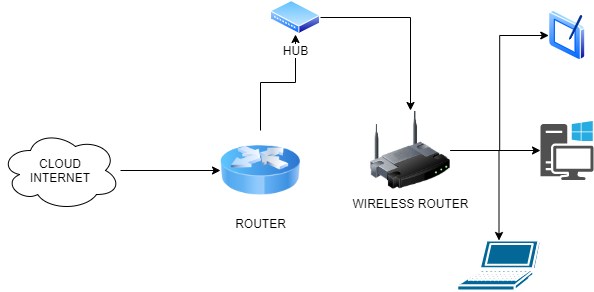
\includegraphics[width=0.4\textwidth]{1.png}
    \caption{Wireless Network}
\end{figure}

Wireless Network atau biasa yang dikenal dengan Wi-Fi merupakan jaringan nirkabel yang digunakan
untuk mengkoneksikan dari satu perangkat ke perangkat lainnya ,
contoh nya Handphone,Laptop,Personal Computer(PC)
ke router jaringan yang sudah disambungkan internet pada port yang disediakan . biasa nya Wireless Network  
erat hubungannya dengan bidang telekomunikasi, teknologi informasi, dan teknik komputer dan jaringan 



Ada banyak jenis jaringan dan cara mengklasifikasikannya. Salah satu cara memandang jaringan adalah dari segi cakupan geografisnya yaitu:

\begin{itemize}
    \item Local Area Network
\end{itemize}

Jaringan area lokal (LAN) dirancang untuk menghubungkan komputer pribadi dan perangkat digital lainnya dalam radius setengah mil atau 500 meter. 
LAN biasanya menghubungkan beberapa komputer di kantor kecil, semua komputer di satu gedung, atau semua komputer di beberapa gedung dalam jarak dekat.
Sistem operasi LAN yang paling umum adalah Windows, Linux, dan lain-lain

\begin{itemize}
    \item Wide Area Networks (WAN)
\end{itemize}
Wide area networks (WAN) menjangkau jarak geografis yang luas (seluruh wilayah, negara bagian, benua, atau seluruh dunia). 
WAN yang paling universal dan kuat adalah Internet.
Komputer terhubung ke WAN melalui jaringan publik, seperti sistem telepon atau sistem kabel pribadi, atau melalui leased line atau satelit. 
Jaringan area metropolitan (MAN) adalah jaringan yang mencakup area metropolitan, biasanya kota dan pinggiran kota utamanya. 
Lingkup geografisnya berada di antara WAN dan LAN.

\begin{itemize}
    \item Metropolitan Area Network (MAN)
\end{itemize}
MAN atau Metropolitan Area Network mencakup area yang lebih besar daripada LAN dan area yang lebih kecil dibandingkan dengan WAN.
Ini menghubungkan dua atau lebih komputer yang terpisah tetapi berada di kota yang sama atau berbeda. 
Ini mencakup area geografis yang luas dan dapat berfungsi sebagai ISP (penyedia layanan internet).
MAN dirancang untuk pelanggan yang membutuhkan konektivitas berkecepatan tinggi.
Kecepatan MAN berkisar dalam hal Mbps. Sulit untuk merancang dan memelihara Jaringan Area Metropolitan. 
Toleransi kesalahan dari MAN lebih sedikit daripada LAN dan juga ada lebih banyak kemacetan di jaringan.
Kecepatan transfer data dan penundaan propagasi dari MAN adalah moderat.

\begin{itemize}
    \item Personal Area Network (PAN)
\end{itemize}
Mewakili teknologi personal area network wireless seperti Bluetooth (IEEE 802.15) dan Infrared (IR). 
Jaringan ini mengizinkan hubungan peralatan personal dalam suatu area berkisar 12 inchi. 
Bagaimanapun juga Infrared membutuhkan hubungan langsung dan jangkauan yang lebih pendek.~\cite{yudianto2014jaringan}

\subsection{Aplikasi InSSIDer}

InSSIDer adalah software yang digunakan untuk memindai dan mengcapture jaringan dengan parameter utama SSID dalam jangkauan antena Wi-Fi komputer, melacak kekuatan sinyal dari waktu ke waktu, dan menentukan pengaturan keamanan mereka (termasuk apakah dilindungi oleh password atau tidak).
Kelebihan dari inSSIDer ini yaitu melacak area hotspot lebih dari kemampuan wireless card PC atau laptop dan juga menampilkan secara real time grafik amplitudo dari access point sehingga dapat diketahui kualitas dan kekuatan sinyal Wi-Fi tersebut. Namun inSSIDer ini juga memiliki kekurangan yaitu bahwa inSSIDer ini tidak bisa menampilkan IP address mana saja yang sedang terhubung dengan access point.


\section{Analisa Jaringan Wireless}
Pada sesi ini dijelaskan analisa jaringan yang ada di kampus Institut Teknologi Batam , ini merupakan analisa dari mahasiswa
pada hotspot wireless yang ada disekitar kampus . 

\begin{figure}[h]
    \centering
    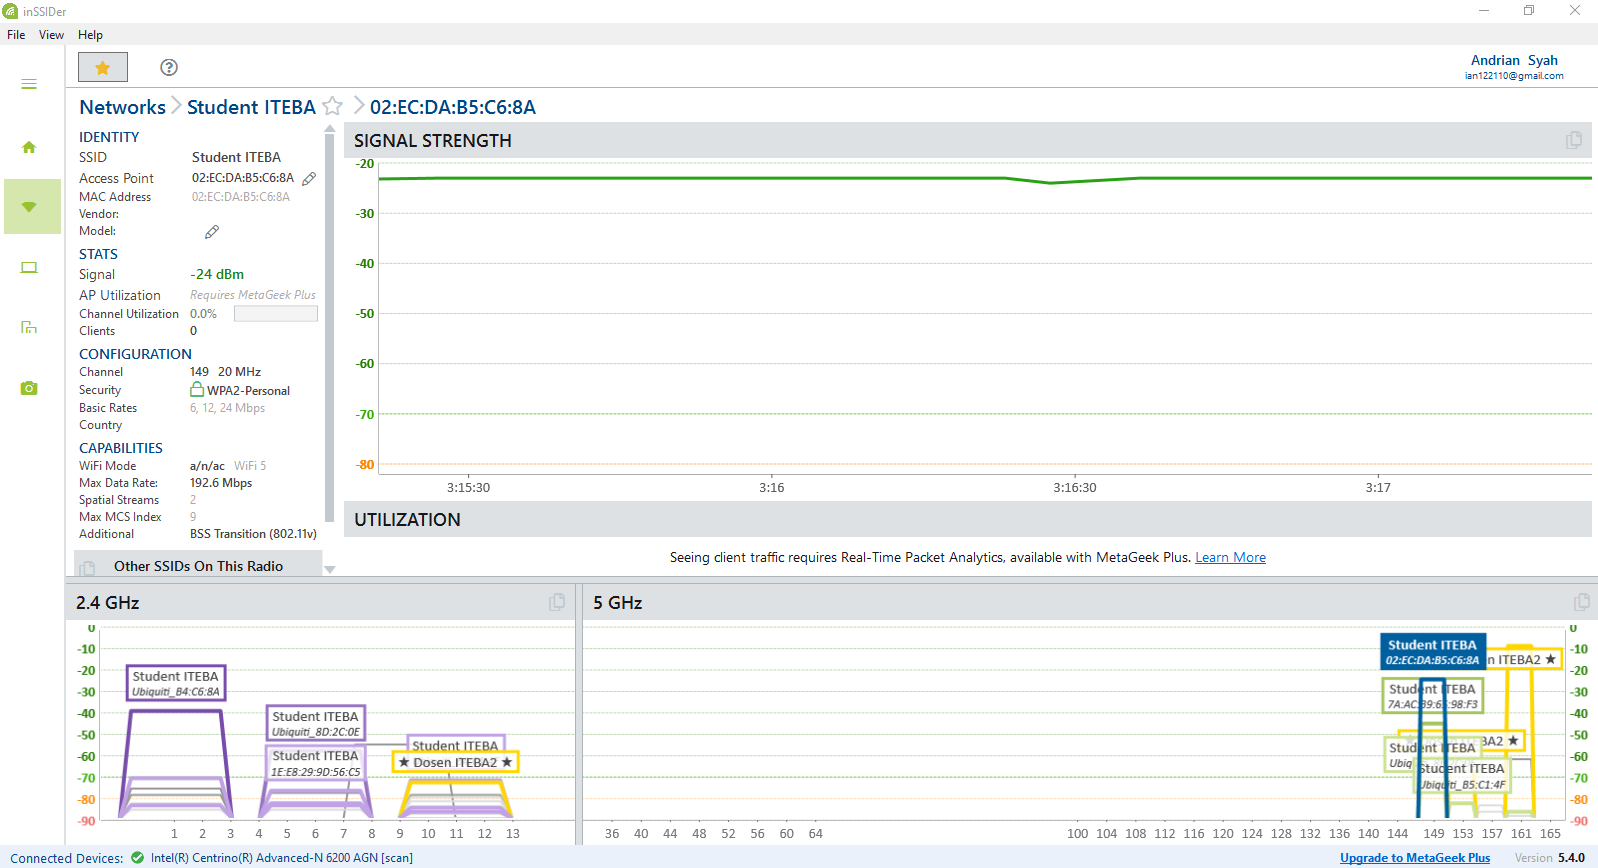
\includegraphics[width=0.5\textwidth]{2.png}
    \caption{Student Iteba hotspot}
\end{figure}

disini terlihat bahwasan nya wifi Student Iteba Mempunyai Kekuatan sinyal sebesar -24 dbm yang dimana sinyal tersebut dikatakan lemah menurut
grafik sinyal yang ada pada gambar dibawah ini .

\begin{figure}[h]
    \centering
    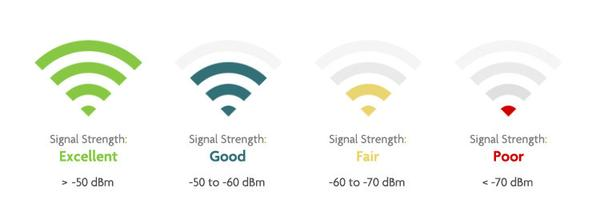
\includegraphics[width=0.5\textwidth]{3.jpg}
    \caption{Grade sinyal wifi}
\end{figure}

karena banyak nya akses point yang digunakan memungkinkan keadaan jika user berpindah , maka device menuju wireless yang akan terhubung,
dan apabila sinyal terhalang oleh tembok maka akan menghasilkan kekuatan sinyal yang lemah , pada saat itu pengetesan dilakukan didalam ruangan
perpustakaan iteba yang didalam nya memiliki perangkat yang dimana kami lihat merupakan sebuah repeater antar jaringan nirkabel .
dapat dilihat pada grafik dibawah ini yang menunjukan banyak nya access point yang bernama Iteba Student yang di double SSID pada perangkat dengan nama SSID
Dosen Iteba , Terlihat dari channel yang digunakan sama dan bahkan pada saat di tinjau melalui aplikasi inSSIDer bahwa SSID tersebut bertumpukan menggunakan 2.4 Ghz dan 5 Ghz.~\cite{arnomoanalisis}

\begin{figure}[h]
    \centering
    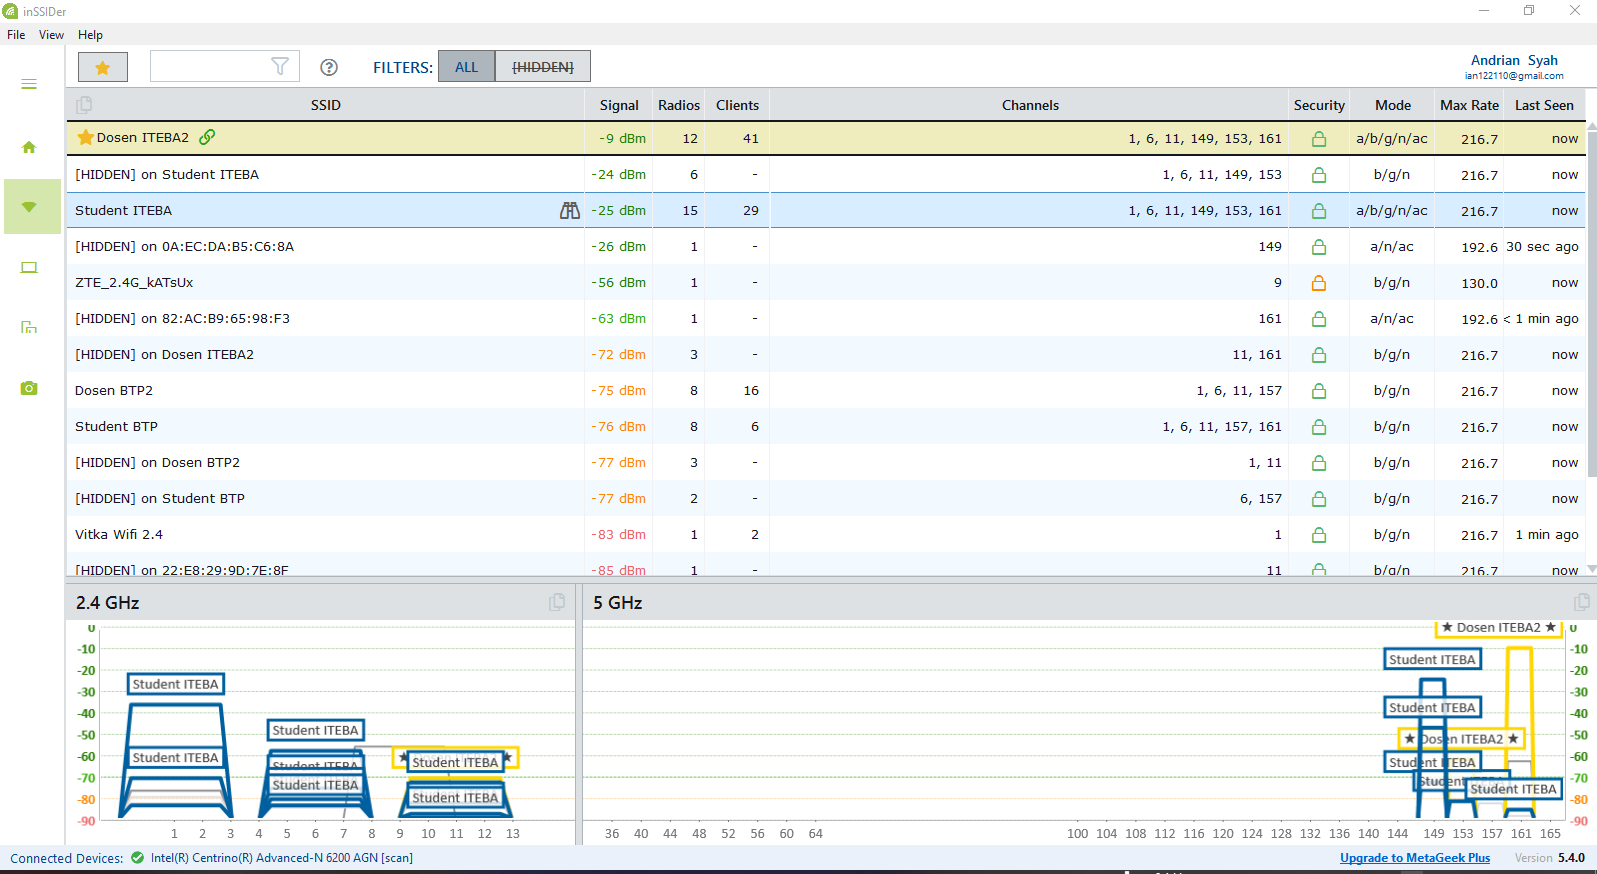
\includegraphics[width=0.5\textwidth]{4.png}
    \caption{Grade sinyal wifi}
\end{figure}



\section{Hasil dan Pembahasan}

Dari hasi analisa jaringan wireless yang dilakukan pada lingkungan kampus
institut teknologi batam yaitu pada saat kami berjalan menuju lantai 2 di area kampus iteba , jaringan akan berpindah
ke akses point terdekat dengan SSID yang sama , karena penggunaaan repeater yang ada dikampus yang menyebabkan apabila terjadi permasalahan
pada pusat jaringan atau Router Utama maka akan terjadi lost koneksi pada setiap semua repeater yang ada .
disini kami juga mencoba kecepatan internet pada SSID Iteba Student menggunakan aplikasi SpeedTest By Ookla

\begin{figure}[h]
    \centering
    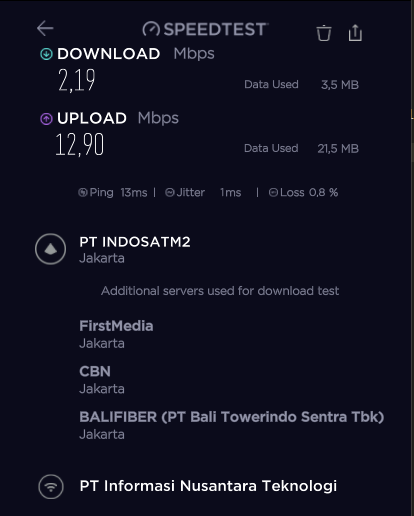
\includegraphics[width=0.2\textwidth]{5.png}
    \caption{SpeedTest Jaringan Internet}
\end{figure}

\vspace{5cm}


pada gambar diatas dapat dilihat kecepatan internet yang di dapat untuk Download hanya mencapai 2,19 Mbps Sedangkan untuk upload  yang
di dapatkan yaitu 12.90 Mbps ini ditest dengan adanya penghalang dinding yang dimana dinding menyebabkan transmisi sinyal menjadi lemah , 
sehingga akses internet yang digunakan menjadi rendah , berikut ini merupakan hasil pengetesan diarea access point terdekat tanpa penghalang

\begin{figure}[h]
    \centering
    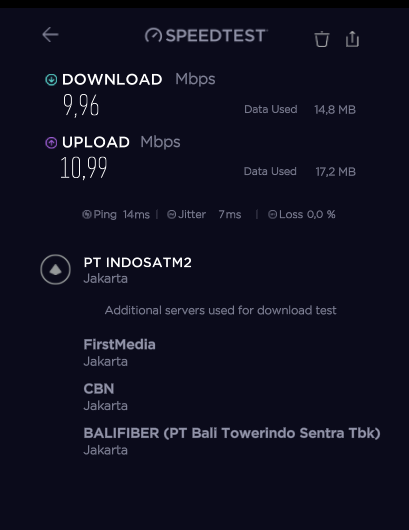
\includegraphics[width=0.2\textwidth]{6.png}
    \caption{SpeedTest Jaringan Internet}
\end{figure}


\section{Kesimpulan}
Dapat disimpulkan bahwa saat pengetesan menggunakan aplikasi InSSIDer kekuatan sinyal juga mempengaruhi transmisi data yang dimana ini menggunakan internet,
sehingga ada nya perbedaan pada saat ada nya penghalang sewaktu pengetesan dan tidak adanya penghalang saat pengetesan , beberapa keunggulan dan kekurangan dari wireless network 
sangat mungkin ada , karena pada dasarnya manusia menciptakan sesuatu hal yang belum sempurna namun dari pernyataan tersebut bahwa manusia membuat perangkat nirkabel untuk memudahkan pengaksesan 
tanpa menggunakan perantara kabel saat terkoneksi di device , perangkat hardware pada device juga mempengaruhi kekuatan sinyal , karena apabila hardware penangkap sinyal yang ada pada suatu 
komputer sudah usang atau sudah rusak , maka sinyal transmisi yang dihasilkan akan lebih jauh menurun .

% referensi %%%%%%%%%%%%%%%%%%%%%%%%%%%%%%%%%%%%%%%%%%%%%%%%
\bibliographystyle{IEEEtran}
\bibliography{referensi}


\end{document}